%%%%%%%%%%%%%%%%%%%%%%%%%%%%%%%%%%%%%%%%%%%%%%%%%%%%%%%%%%%%%%%%%%%%%%%%
% Created 2020-09-30 Wed 15:22
% Intended LaTeX compiler: pdflatex
\documentclass[10pt,t]{beamer}
\usepackage[utf8]{inputenc}
\usepackage[T1]{fontenc}
\usepackage{graphicx}
\usepackage{grffile}
\usepackage{longtable}
\usepackage{wrapfig}
\usepackage{rotating}
\usepackage{amsmath}
\usepackage{textcomp}
\usepackage{amssymb}
\usepackage{capt-of}
\usepackage{hyperref}
\usepackage{pdfpages}
%\usepackage{scrextend}
%\usepackage{lipsum}
\input beamer_setup
\usetheme{metropolis}
\metroset{titleformat title=allcaps}
\renewcommand{\UrlFont}{\small\tt}
\renewcommand*{\UrlFont}{\footnotesize}
\tolerance=1000
\setlength{\leftmargini}{3pt}
% \setbeamersize{
%   text margin left=3mm,
%   text margin right=3mm,
% }
%---------------------------------------------------------------------------------------------
\author{S. Machado}
\date{\today}
\title{\large Twenty Years of Infrared Hyperspectral Satellite Measurements}
\subtitle{\footnotesize{From Spectroscopy to Climate Workshop \\ \vspace{-0.07in} Princeton Center for Theoretical Sciences}}
\date{\vspace{0.1in}\footnotesize{August 22-24,2022, Princeton NJ \vfill}}
\author{Sergio DeSouza-Machado\inst{1}, Joao Teixeira\inst{2}, and L. Larrabee Strow\inst{1}}
\institute{\inst{1}UMBC Physics Department \and \inst{2}NASA Jet Propulsion Laboratory}
%---------------------------------------------------------------------------------------------
\begin{document}
\maketitle
%---------------------------------------------------------------------------------------------
\begin{frame}
  \frametitle{Overview}  
  \begin{itemize}
  \item Hyperspectral infrared satellite sounders (since 2002)
    \begin{itemize}
    \item AIRS, IASI, CrIS, etc
    \item Major uses of these sounders
    \item Timelines
    \end{itemize}
  \item Spectroscopy for infrared sounders
    \begin{itemize}
    \item Fundamental liens
    \item Radiative transfer: hierarchy of models
    \item Clouds ...
    \end{itemize}
  \end{itemize}
  \begin{itemize}
  \item Longterm trends and feedbacks from AIRS: Various Approaches
  \item Long term radiance dataset for climate: CHIRP (in Amazon Cloud)
  \end{itemize}
\end{frame}
% ---------------------------------------------------------------------------------------------
\begin{frame}
  \frametitle{Possible Take-Homes}
  \begin{itemize}
  \item Future research with these sensor concentrating on processes and climate
  \item Direct use of radiances by the climate community:
    \begin{itemize}
    \item Retain accuracy and traceability of results to the raw data
    \item Simple algorithms that can be executed quickly (cloud computing)
    \item Non-standard products: cloud PDFs, fires, etc.
    \item Trends and anomalies
    \end{itemize}
    \item How to handle practical issues: data access, RTAs, etc.
  \end{itemize}
\end{frame}

%------------------------------------------------------------------------

\begin{frame}[shrink=2]{Spectroscopy}
\vspace{-0.1in}

\begin{itemize}
  \item HITRAN line parameter released every 4 years
  \item H2020 : self consistent changes to O3 line intensities (MW to UV) $\Delta BT(K) \sim 0.5K$ at 10 um
  \item Uncertainty estimates : $\delta(BT) \sim$ 0.2 K at TOA  
  \item Line mixing models; speed dependent Voigt line shapes used in other spectral regions
  \item AER : \textcolor{red}{new WV continuum in Fall 2022 (TIR region); H2020 \cd/\methane linemixing}
  \item GEISA database (France) is very similar to HITRAN
  %\item NLTE mostly affects the 4.3 um \cd band (nadir sounding)
  %\item Manuel Lopez Puertas (Granada, Spain) has developed models upper atmosphere NLTE vibrational temperatures
  %\item UMBC developed a fast model using this database
  %\item We don't worry too much about strat/meso temperatures and atmospheric concentrations (cannot see with nadir sounders)
\end{itemize}
\end{frame}

%%%%%%%%%%%%%%%%%%%%%%%%%%%%%%%%%%%%%%%%%%%%%%%%%%%%%%%%%%%%%%%%%%%%%%%%
\begin{frame}{Impact of Spectral Uncertainties ($\Delta$ (BT) at TOA)}

\begin{columns}
\begin{column}{0.55\columnwidth}
%\begin{block}{Perturbations}
wavenumber, pressure line shift unc \newline
GEISA vs HITRAN  
%\end{block}
\end{column}

\begin{column}{0.55\columnwidth}
\vspace{0.25in} $\le$ 0.1 K RMS differences
\end{column}
\end{columns}

%%%%%%

\vspace{0.25in}
\begin{columns}
\begin{column}{0.55\columnwidth}
\begin{block}{Spectroscopic Database}
LBLTMv12.8 15 \um \cd line mixing versus \newline
LBLRTM 12.4 (red) UMBCLBL (blue) \newline
\textcolor{red}{Integral over wavenumber would give similar fluxes}
\end{block}
\end{column}

\begin{column}{0.55\columnwidth}
\begin{figure}
\begin{center}
%\includegraphics[width=0.45\textwidth]{../../SUBMITPAPERS/PAPER1_KCARTA/GEISA_HTRAN/hitran_geisaV2.pdf}
%\includegraphics[width=1.005\textwidth]{../../SUBMITPAPERS/PAPER1_KCARTA/GEISA_HTRAN/co2_linemix_flavorsV2.pdf}
\includegraphics[width=1.005\textwidth]{NEWFIGS/co2_linemix_flavorsV2.pdf}
\end{center}
\end{figure}
\end{column}
\end{columns}

\end{frame}

%%%%%%%%%%%%%%%%%%%%%%%%%%%%%%%%%%%%%%%%%%%%%%%%%%%%%%%%%%%%%%%%%%%%%%%%

\begin{frame}[shrink=2]{Radiative Transfer codes}

\emph{Line by line codes : accuracy}
\vspace{-0.1in}
\begin{itemize}
  \item Latest HITRAN databases; accurate; too slow for operational use
  \item LBLRTM (AER) MT-CKD continum, \cd/\methane line mixing, MW $\rightarrow$ UV
  \item \textcolor{red}{kCARTA (UMBC)} \emph{HITRAN (2020), MT-CKD 3.2,\cd/\methane linemixing from LBLRTM, 
        605-2830 \wn at 0.0025 \wn resolution (25 sec), 15-44000 \wn (5 min), jacobians, 
        fluxes, scattering}
\end{itemize}

\emph{Fast Models : speed}
\vspace{-0.1in}
\begin{itemize}
  \item Parametrized fast codes for clear sky cloud clearing retrievals
  \item \textcolor{red}{SARTA (UMBC)} \emph{used by NASA and NOAA for operational L2 retrievals of AIRS, CrIS, IASI}
  \item PCRTM (NASA Langley)
  \item RTTOVS (ECMWF) Data Assimilation
  \item Sigma IASI (U. of Basilicata, Italy) 
\end{itemize}
\end{frame}

%%%%%%%%%%%%%%%%%%%%%%%%%


\begin{frame}[shrink=2]{Clouds and Aerosols}

\begin{itemize}
  \item Dust (4um), water (20 um), ice (20-100 um) affects TIR
  \item DISORT (Stamnes et. al. 1988) : Very accurate, but slow
  \item Parameterization for LongWave Scattering (Chou et. al 1999) : Very fast, about 2 K errors
  %\item Successive Orders of Scattering : mostly used for NIR/Vis (to my knowledge)
  \item PCLSAM fix (Tang. et. al 2018) : Needs more work
  \item Complex cloud models (Maximum Random Overlap) give smooth heating profiles, multiple sub pixels are computationally costly
  \item Simple cloud models (TwoSlab) are fast and quite accurate, spikes at cloud slab boundaries
%  \item RRTM (AER) has in-built fast RTA for flux calculations, handles scattering, 3-4 gaussian angles
%  \item ecRad (Robin Hogan, ECMWF) developed flux model for ECWMF
\end{itemize}
\end{frame}

%%%%%%%%%%%%%%%%%%%%%%%%%

\begin{frame}[shrink=2]{Operational Retrievals}
\vspace{-0.11in}

\emph{Typical Hyperspectral Sounder}
\vspace{-0.1in}
\begin{itemize}
  \item About 2000+ channels, resolution about 0.5-2 cm-1, 15 km diameter footprint
  \item 1.30 am/pm equator crossing time, twice daily views of Earth, 16 day repeat cycle
  \item 90 xtrack x 135 atrack spectra every 6 minutes
  \item Roughly \textcolor{red}{2.92 million  allsky spectra daily x 20 years!}
\end{itemize}

\vspace{0.10in}

\emph{Operational Retrievals : Cloud Clearing}
\vspace{-0.1in}
\begin{itemize}
  \item reduces spatial resolution from 15 km to 3x3 or 45 km
  \item ``increases'' spectral noise, and hence retrieval uncertainty
  \item fails when scenes are uniform eg MBL, dust, clear
  \item \textcolor{red}{T(z), WV(z), surface temp, trace gases, clouds, emissivity}
  \item AIRS v7 : neural network first guess, 2 sec/FOR, Lots of QA, 
  \item NOAA CLIMCAPS MERRA2 first guess, simpler QA, 0.7 sec/FOR
  \item Single Footprint? Artificial Intelligence?
\end{itemize}

\end{frame}

%%%%%%%%%%%%%%%%%%%%%%%%%%%%%%%%%%%%%%%%%%%%%%%%%%%%%%%%%%%%%%%%%%%%%%%%

%---------------------------------------------------------------------------------------------
% % ---------------------------------------------------------------------------------------------
% \begin{frame}
% \frametitle{Possible Take-Homes}  
%   \begin{itemize}
%   \item Do your science as ``close to the radiances'' as possible.  Products have a-priori information that must be properly accounted for, which can be difficult.
%   \item What questions can best be studied with the satellite radiance record?  
%   \item The data is available in the Amazon cloud and will soon be in a cloud-native format for quick processing by anyone
%   \item Extremely fast processing is possible, esp. compared to thermal imagers
%   \item Help us persuade NASA that these combined NASA/NOAA mission data are important and need preservation and maintenance.  Both NASA missions providing hyperspectral radiances will cease in the next few years, the NOAA missions (JPSS) will continue.
%   \end{itemize} 
% \end{frame}
% %---------------------------------------------------------------------------------------------
% \begin{frame}
% \frametitle{``Operational'' Hyperspectral Infrared Satellite Sounders}
% \begin{columns}[T]

%   \begin{column}{0.75\columnwidth}
%   \begin{itemize}
%   \item \textbf{AIRS:} Grating spectrometer, 2378 channels, $\nu / \Delta \nu \approx 1200$
%   \item \textbf{IASI/IASI-NG:} Interferometer, 8461/16922 channels, $\Delta \nu = 0.50/0.25 cm^{-1}$
%   \item \textbf{CrIS: }NASA SNPP-CrIS/NOAA JPSS-1-4, 2235 channels, $\Delta \nu \approx 0.625-1 cm^{-1}$
%   \end{itemize}

% \begin{small}  
% Noise levels $\approx$ 0.05-0.2K, footprints $\approx$ 15 km, nearly full earth coverage 2X per day (2-3 million obs)
% \end{small}  

% \end{column}

% \begin{column}{0.25\columnwidth}
%   \vspace{-0.15in}
%   \begin{block}{AQUA Satellite}
%   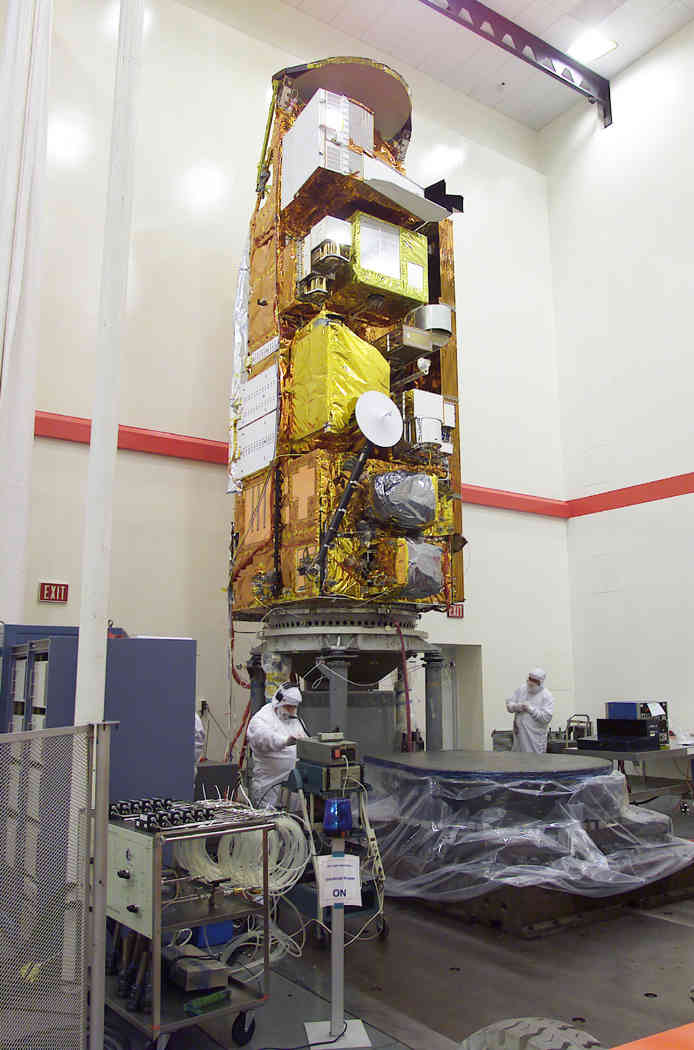
\includegraphics[width=1.1\textwidth]{./aqua.jpg}
% \end{block}
% \end{column}
% \end{columns}

% \begin{footnotesize}
% \begin{tabular}{lll}
% AIRS & 2002 - 202X?? & 1:30 orbit\\
% \hline
% CrIS & 2012 - 204X? & 1:30 orbit\\
% \small 1 SNPP-CrIS, 4 on JPSS &  & \\
% \hline
% IASI & 2007 - 204X? & 9:30 orbit\\
% \small 3 each on METOP-A and METOP-SG series &  & \\
% \hline
% CHIRP (AIRS+CrIS) & 2002 - 204X & 1:30 orbit\\
% "Virtual" L1c for climate &  & \\
% \end{tabular}
% \end{footnotesize}

% \end{frame}
%---------------------------------------------------------------------------------------------
% I need to put in CHIRP, get rid of CrIS-Hamming
\begin{frame}
\frametitle{BT(K) Spectra for IR Sounders}  
\begin{center}
%\includegraphics[width=0.9\linewidth]{../../CONFERENCES/SunClimate2022/Strow_JPL_Apr2022/jpl_min//hyperall_hamming.pdf}
\vspace{-0.05in}
\includegraphics[width=0.8\linewidth]{SunClimate2022/hyperall_hamming.pdf}
\end{center}
\vspace{-0.1in}
\small Major gases: \cd, \water, \ozone, \methane, \nitrous \\
\small Minor gases: CO, CFCs, SO$_2$, NH$_3$, PAN, and many others (+dust)
\end{frame}
%---------------------------------------------------------------------------------------------
\begin{frame}
\frametitle{Measured Radiances and Trends for Clear Scenes}
\centering 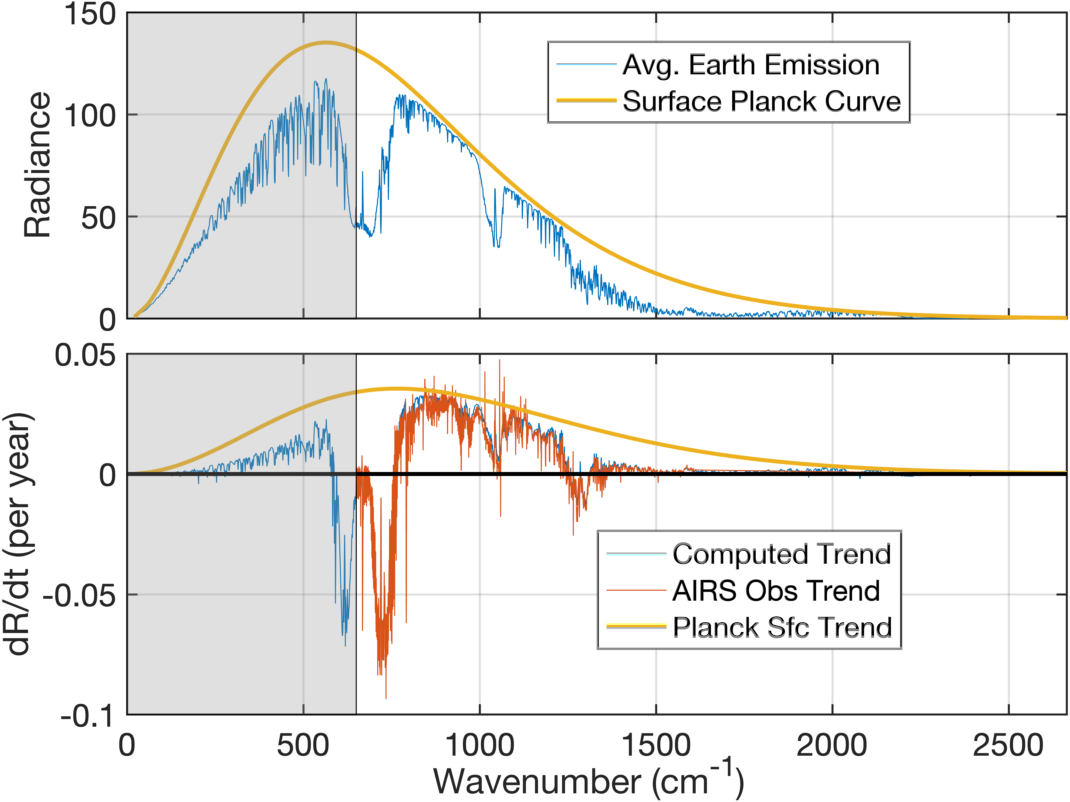
\includegraphics[width=0.7\linewidth]{Figslls/rad_trends_all_cm.png}
\begin{small}
\begin{itemize}
\item Top: Simulated Earth avg. spectrum: 1 \wn spectral response
\item Bottom: 19-year linear trend.  Red obs inverted and then used to compute blue curve.  Used hottest 2\% per 16 days in 3x5 grid.
\item Water trend retrieval robust, but not in ``active'' FIR region for OLR
\end{itemize}
\end{small}
\end{frame}
%---------------------------------------------------------------------------------------------
\begin{frame}
\frametitle{Measured BT Spectra and Trends for Clear Scenes}  
\vspace{-0.03in}
\centering 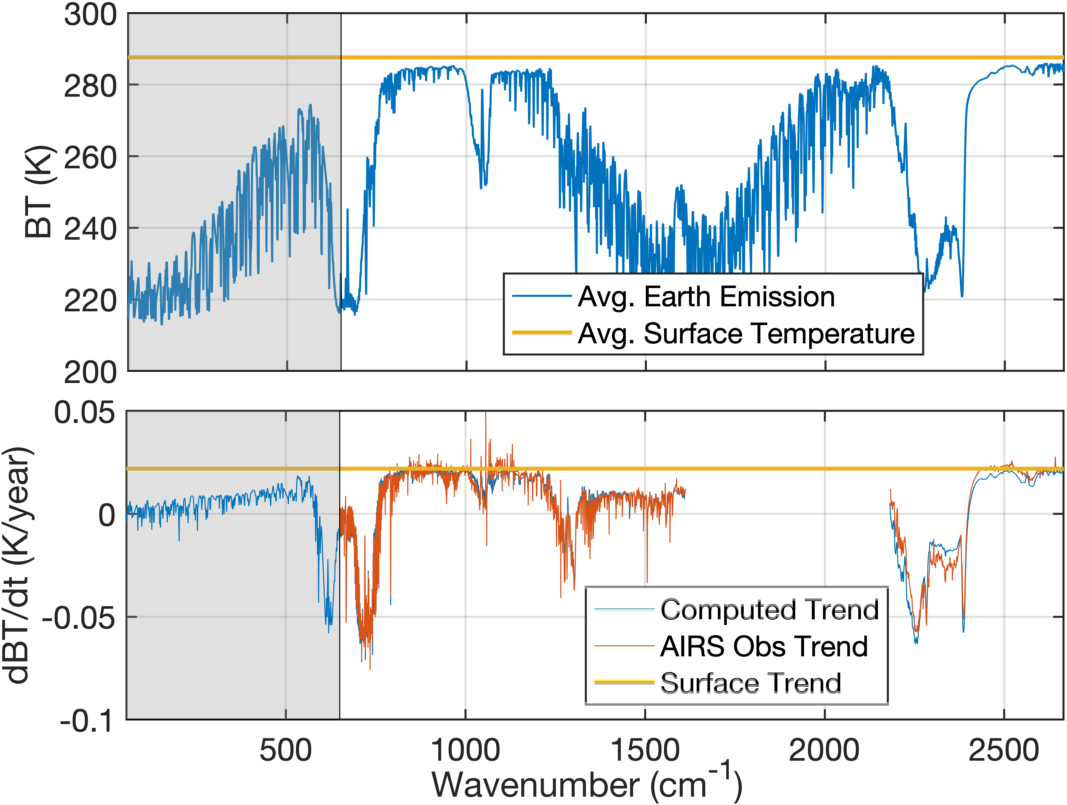
\includegraphics[width=0.7\linewidth]{Figslls/bt_trends_all_cm.png}
\vspace{-0.05in}
\begin{small}
\begin{itemize}
\item Same as previous slide but in BT units.
\item AIRS etc. covers same altitudes that control far-IR emission
\item Highlights water vapor feedback, lowering emission to space
\item Note: Tropospheric warming close to surface temperature warming  
\end{itemize}
\end{small}
\end{frame}

%---------------------------------------------------------------------------------------------
\begin{frame}
  \frametitle{Upwelling Radiance Example}
\vspace{-0.05in}
  \centering 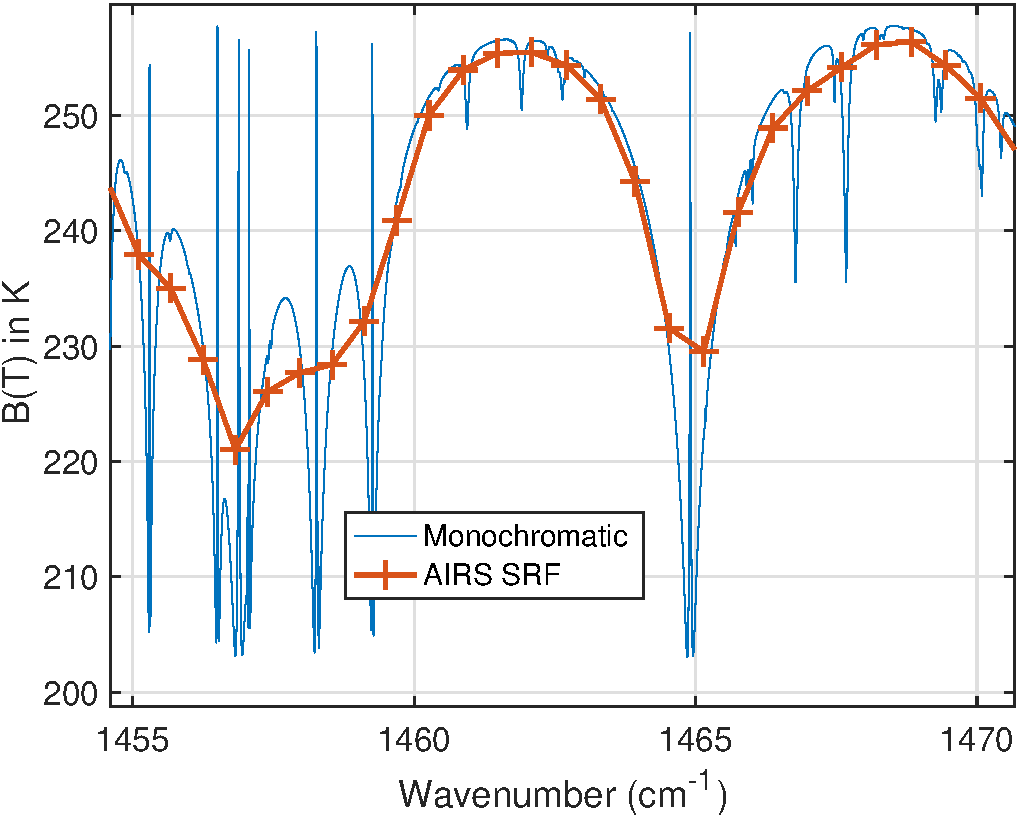
\includegraphics[width=0.75\linewidth]{Figslls/mono1460.pdf}
\vspace{-0.05in}
\begin{small}
\begin{itemize}
  \item Best sounding channels are in-between lines (pressure$^2$ dependence \vspace{-0.03in})
  \item Line centers have stratospheric contributions \vspace{-0.03in}
  \item A further zoom will show a dip from the mesosphere!
  \end{itemize}
\end{small}
\end{frame}
% ---------------------------------------------------------------------------------------------
\begin{frame}
  \frametitle{Radiative Transfer Models}
  \begin{itemize}
  \item Inversion of radiance spectra requires accurate ``fast'' models
  \item These are trained on monochromatic models (LBLRTM, kCARTA)
  \item AIRS/CrIS RTAs:  SARTA (UMBC), PCRTM (NASA/Langley), CRTM (NOAA), OSS (AER), RTTOV(ECMWF)
  \item NWP oriented models often don't have all minor gases
  \end{itemize}
  \begin{block}{Simple Radiative Transfer}
    \centering 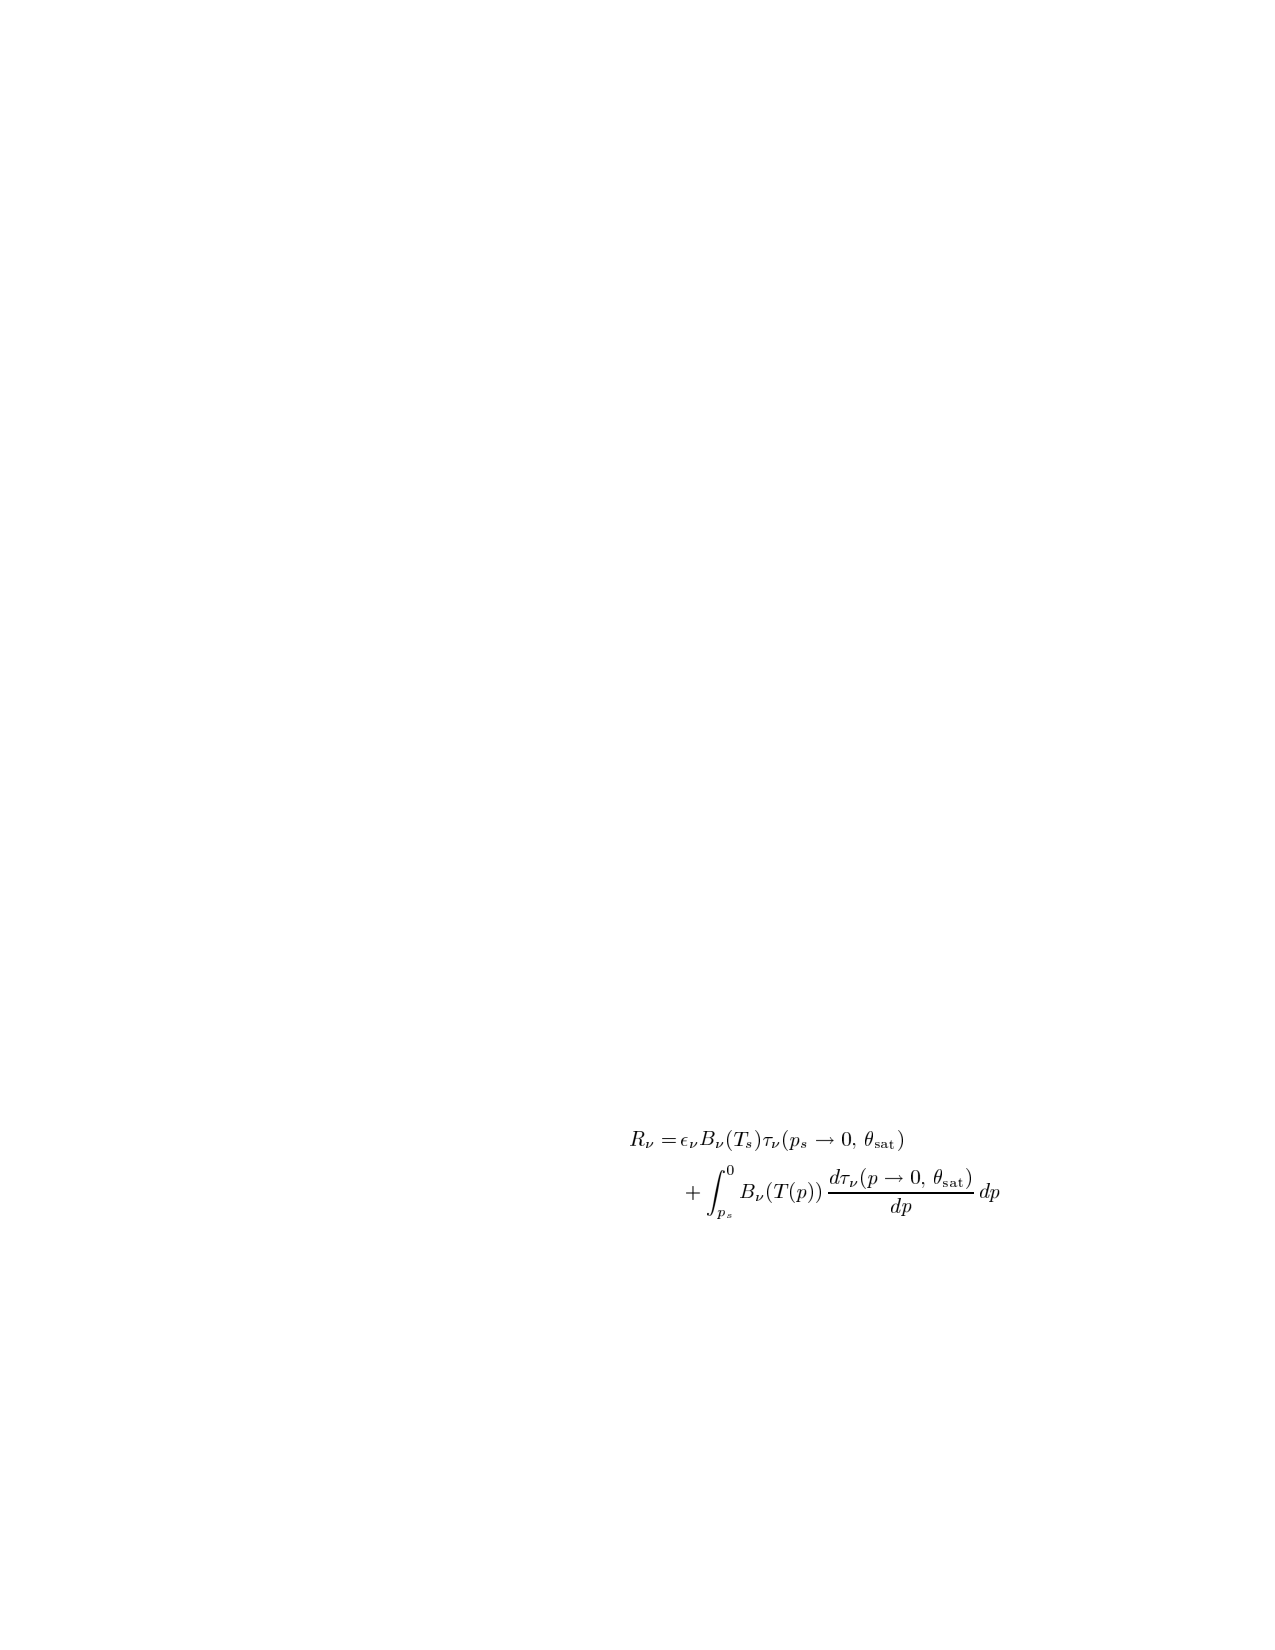
\includegraphics[width=0.55\linewidth]{Figslls/simple_rta.pdf}
   \begin{small}
    \begin{itemize}
    \item $\tau_{\nu}$ extremely complicated and contain the spectroscopy
    \item Spectral lineshapes (and continua) dominate uncertainties
    \item Example: recent work (Hartmann) highighted importance of N$_2$-\water emission for sounding
    \end{itemize}
 \end{small}
  \end{block}
\end{frame}

%---------------------------------------------------------------------------------------------
\begin{frame}
  \frametitle{NWP Forecast Impact: \small (From Marcos Matricardi, ECMWF)}
  \vspace{-0.1in}
  \begin{small}
  \begin{itemize}
  \item NWP users ``pay the bills'' (NCEP, ECMWF, METEO-France, etc.)
  \item They ingest radiances (small subset of channels) for data assimilation
  \item Dynamic bias correction (via sondes, GNSS RO?) removes instrument, RTA, \textit{and} variable CO$_2$ before assimilation.
\end{itemize}
  \end{small}
  \vspace{-0.45in}
  \includegraphics[width=\linewidth,page={13}]{Matricardi_REVEX_2021.pdf}
\end{frame}
%---------------------------------------------------------------------------------------------
\begin{frame}
\frametitle{Climate Model Evaluation}  
\vspace{-0.35in}
\begin{center}
\includegraphics[width=1.01\linewidth,page={10}]{Slides_to_Sergio.pdf}
\end{center}
\end{frame}
%---------------------------------------------------------------------------------------------
\begin{frame}
\frametitle{L2 Retrievals : CLIMCAPS}  
\vspace{-0.35in}
\begin{center}
\includegraphics[width=1.01\linewidth,page={8}]{Slides_to_Sergio.pdf}
\end{center}
\end{frame}
%---------------------------------------------------------------------------------------------
\begin{frame}
\frametitle{Sample Study: ENSO Variability}  
\vspace{-0.35in}
\begin{center}
\includegraphics[width=1.01\linewidth,page={3}]{Slides_to_Sergio.pdf}
\end{center}
\end{frame}
%---------------------------------------------------------------------------------------------
\begin{frame}
\frametitle{AIRS Spectral OLR}  
\vspace{-0.35in}
\begin{center}
\includegraphics[width=1.01\linewidth,page={9}]{Slides_to_Sergio.pdf}
\end{center}
\end{frame}
%---------------------------------------------------------------------------------------------
\begin{frame}
\frametitle{Gravity Waves: Research Based on Raw Radiances}  
\vspace{-0.35in}
\begin{center}
\includegraphics[width=1.01\linewidth,page={2}]{Slides_to_Sergio.pdf}
\end{center}
\end{frame}
%---------------------------------------------------------------------------------------------
\begin{frame}
\frametitle{Night minus Day Surface T Trends}
\vspace{-0.2in}

\begin{columns}
\begin{column}{0.55\columnwidth}
\begin{block}{\footnotesize Warmer Nights parts of N.H.}
\vspace{-0.1in}
\begin{center}
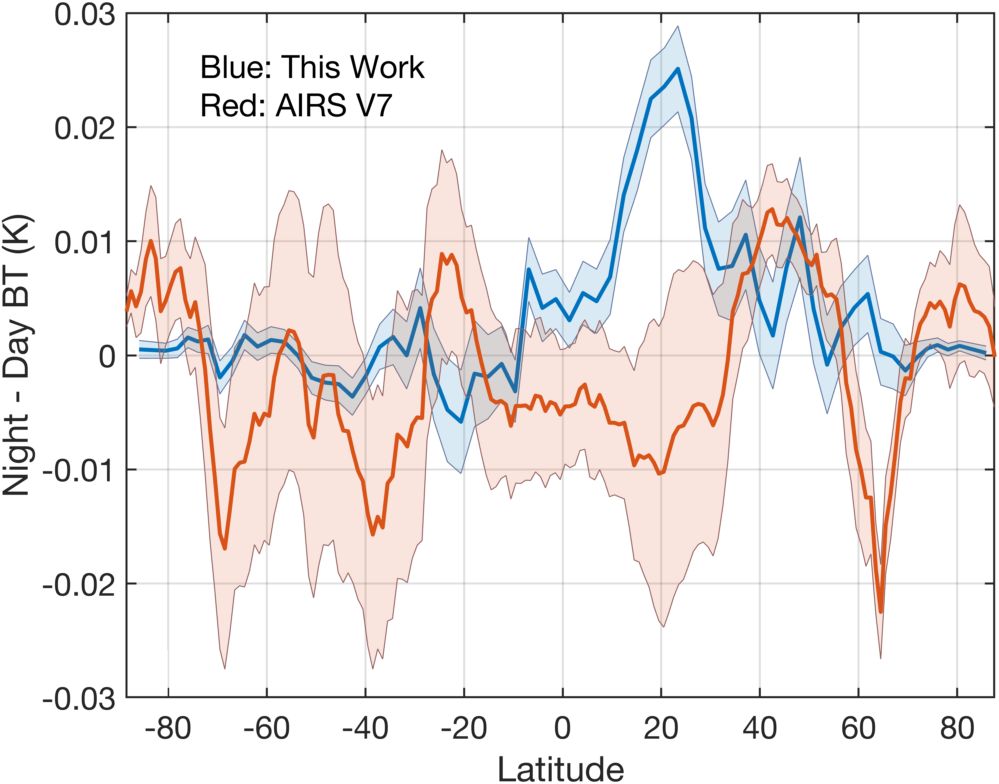
\includegraphics[width=\linewidth]{./Figs21/desc_minus_asc_5pc_hot_bt_trend_with_airs_v7.png}
\end{center}
\end{block}
\end{column}


\begin{column}{0.5\columnwidth}
\begin{block}{\footnotesize Tsurf Anomaly (Warm Pool)}
\vspace{-0.05in}
\begin{center}
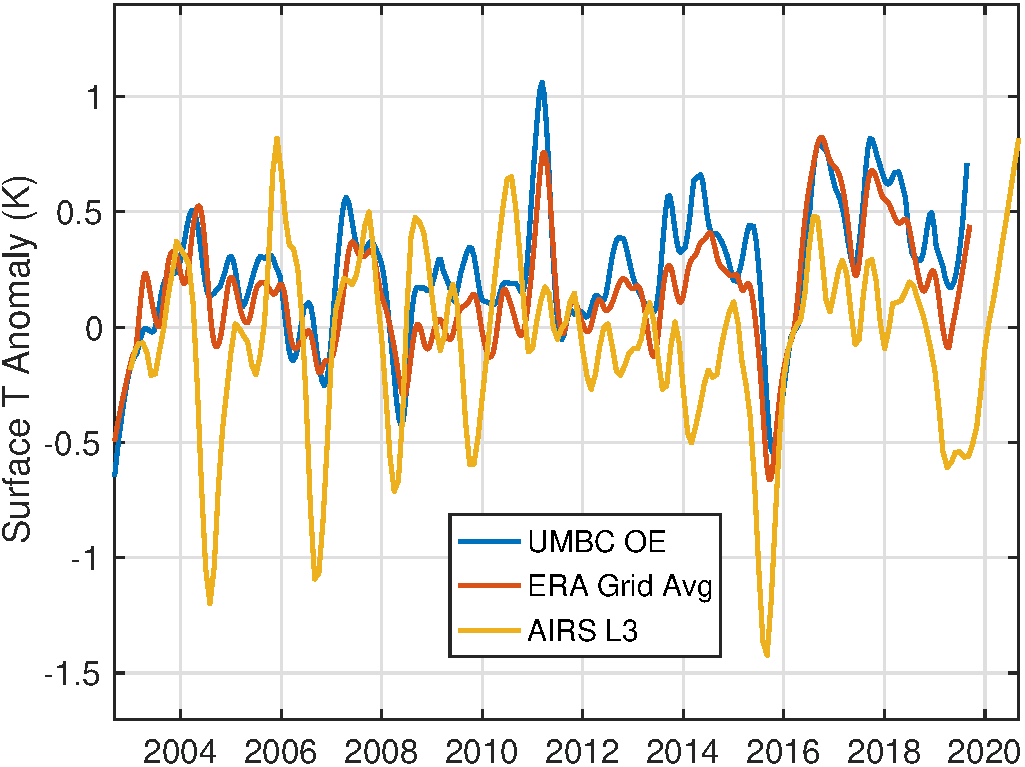
\includegraphics[width=\linewidth]{./Figs21/pro_tsurf_anom.pdf}
\end{center}
\end{block}
\end{column}
\end{columns}

\begin{itemize}
\item Our simple approach shows far less variability in Night-Day surface T trends than AIRS V7
\item Probably due to cloud-clearing issues, see V7 Tsurf anomaly
\end{itemize}
\end{frame}
%---------------------------------------------------------------------------------------------
\begin{frame}
\frametitle{Radiance Trends (18 Yrs): Anomaly Retrieval Closures}
\vspace{-0.35in}

\begin{columns}
\begin{column}{0.55\columnwidth}
\begin{block}{\footnotesize Global Trends: Clear vs All-Sky}
\vspace{-0.1in}
\begin{center}
\includegraphics[width=\linewidth]{./Figs21/global_trends_hottest3pc_and)allsky.pdf}
\end{center}
\end{block}
\end{column}


\begin{column}{0.5\columnwidth}
\begin{block}{\footnotesize Tsurface Global Anomaly}
\vspace{-0.05in}
\begin{center}
\includegraphics[width=\linewidth]{./Figs21/global_bt1231_anomaly.pdf}
\end{center}
\end{block}
\end{column}
\end{columns}

\vspace{-0.1in}
\small
\begin{itemize}
\item 3\% hot sampling trends almost same as all-sky
\item Zonally averaged uncertainties (inter-annual variability) \textasciitilde{}0.05K/Decade
\begin{itemize}
\item Best AIRS stability: \textasciitilde{}0.02K/Decade
\item BUT, in the water band possible errors up to \textasciitilde{}0.04K/Decade due to instrument radiometric shift
\end{itemize}
\end{itemize}
\end{frame}
%---------------------------------------------------------------------------------------------
\begin{frame}
\frametitle{Remove Minor Gas Trends (18 Years)}
\vspace{-0.1in}

\begin{center}
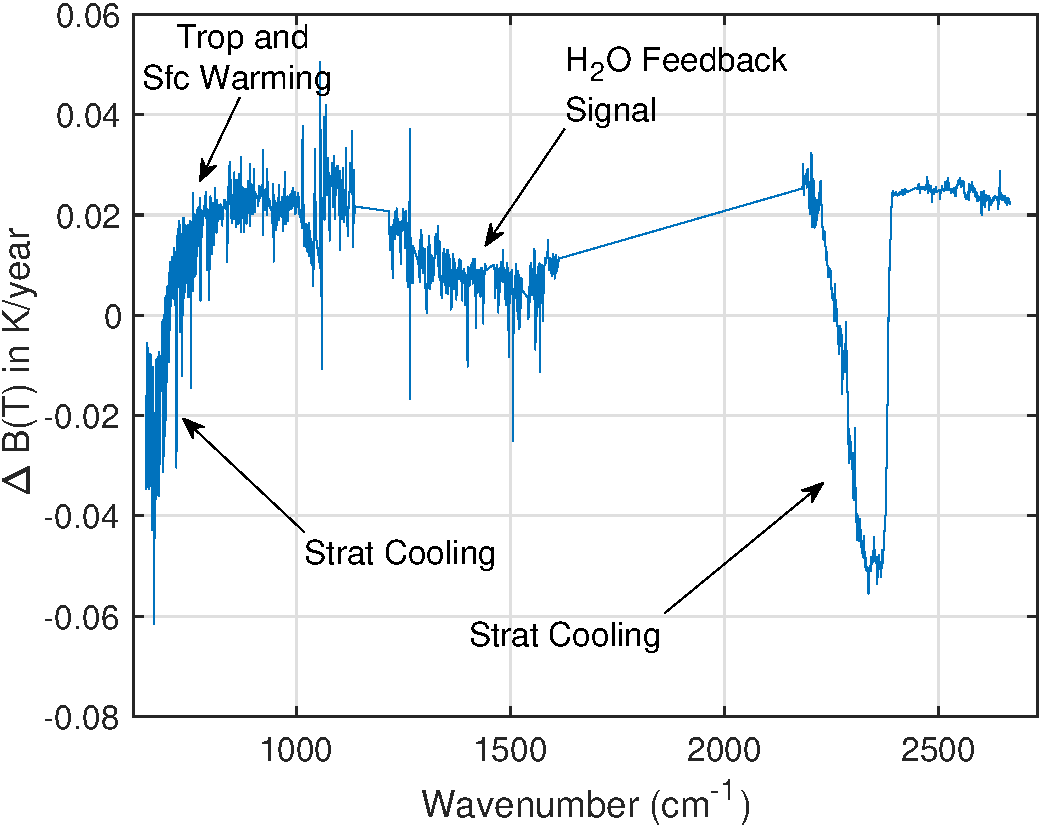
\includegraphics[width=0.7\linewidth]{./Figslls/global18year_forcing_removed.pdf}
\end{center}

\vspace{-0.15in}
\begin{small}
\begin{itemize}
\item \(\Delta\) T troposphere and surface quite similar
\item \water greenhouse effect evident.  Is RH \textasciitilde{} 0?
\item Stratospheric cooling very evident
\item Single 3x5 grid cell inter-annual variability \textasciitilde{}0.03K/year
\end{itemize}
\end{small}
\end{frame}
%---------------------------------------------------------------------------------------------
\begin{frame}
\frametitle{Science Uses of Hyperspectral IR}  
\begin{itemize}
  \item Weighting functions gives high vertical resolution atmospheric sounding information which captures 
         T(z) from surface to stratosphere ($\sim$ 1 km), WV(z) from surface to UT/LS, \ozone, \cd, \methane etc
  \item Trace Gas Studies/Atmospheric Composition
  \item Climate Process Studies and Radiance Trending
  \end{itemize}
\end{frame}
%---------------------------------------------------------------------------------------------
\begin{frame}
\frametitle{Climate Studies and The Future}  
\begin{itemize}
  \item AIRS record : 20 years (started 2002/09, still working well)  
  \item Aqua platform running out of power by 2026 (flight maneuvers + come down safely), slowly de-orbit from A-Train
        but still provide data at different time than 1.30 am/pm
  \item NASA may turn mission off in couple years (budget pressure)
  \item CrIS (NOAA) already in orbit for weather purposes \textcolor{red}{CHIRP product for continuity}
\end{itemize}
\end{frame}
%---------------------------------------------------------------------------------------------
\begin{frame}
\frametitle{Overall Approach}  
\begin{itemize}
\item Driven by Level 2 + Time \(\neq\) Climate
\item Full sampling not required for climate
\item Manipulate data in radiance space "as long as possible" before retrievals
\item Reduce sensitivity to calibration and RTA bias (radiance anomalies)
\item Optimal estimation retrievals regularized more by smoothing than a-priori
\item Develop analysis approaches that encourage more researchers to use radiances, rather than complicated Level 2 products for climate research, with quick turnaround.
\end{itemize}
%Working to provide CHIRP data on GES DISC AWS Cloud storage in format that allows high-speed I/O for end-user processing of radiances.
\end{frame}
%---------------------------------------------------------------------------------------------
\begin{frame}
\frametitle{AIRS Stability Validation (Clear Ocean Scenes Time Series)}  
\vspace{-0.1in}
\begin{center}
%\includegraphics[width=0.65\linewidth]{../../CONFERENCES/SunClimate2022/Strow_JPL_Apr2022/jpl_min//yung/Figs/Pdf/fig10.pdf}
\includegraphics[width=0.65\linewidth]{SunClimate2022/fig10.pdf}
\end{center}

\vspace{-0.05in}
\footnotesize
\begin{itemize}
\item \cd trend (using 400 "good" channels) suggests stability:  -0.023 \textpm{} 0.009 K/decade.  Picks up ENSO related variations in \cd growth at the 0.04K with good S/N
\item \methane and \nitrous trends exhibit small offsets (known events, fixable)
\item (AIRS - GHRSST) SST trends:):  -0.022 \textpm{} 0.012 K/decade
\item This approach provides strong evidence of inherent radiometric stability at the climate level
\end{itemize}
\end{frame}
%---------------------------------------------------------------------------------------------
\begin{frame}
\frametitle{Radiance Sampling}  
\begin{itemize}
\item Early testing shows identical surface T trends with 1\%, 3\%, 5\%, and 10\% hottest scenes per 16-day gridded lat/lon cell (3x5 lat/lon).
\item Will this sampling provide accurate profile trends?
\item Careful sampling of cloudier scenes does not preclude retrievals, just more care in cloud parameter a-priori values and parameterization
\begin{itemize}
\item Hyperspectral IR retrievals really need footprint matched cloud parameters from MODIS (like CERES uses).  Univ. Wisconsin has already generated this product for CrIS from VIIRS!
\end{itemize}
\item Subsequent results used 3\% surface T sampling (from 1231 \wn channel)

\vspace{0.1in}
\end{itemize}

Trend retrievals in next few slides take \textasciitilde{}1 hour max, so reprocessing is trivial.\\
  \vspace{0.1in}
Resampling (say for fixed cloud forcing) takes \textasciitilde{}2 days.  
\end{frame}
%---------------------------------------------------------------------------------------------
\begin{frame}
\frametitle{Global IR Radiance Trends and Surface-T Anomalies}  
\vspace{-0.35in}

\begin{columns}
\begin{column}{0.55\columnwidth}
\begin{block}{\footnotesize Global Trends: Clear vs All-Sky}
\vspace{-0.1in}
\begin{center}
%\includegraphics[width=\linewidth]{../../CONFERENCES/SunClimate2022/Strow_JPL_Apr2022/jpl_min//Figs1/Pdf/global_trends_hottest3pc_and)allsky.pdf}
\includegraphics[width=\linewidth]{SunClimate2022/global_trends_hottest3pc_and)allsky.pdf}
\end{center}
\end{block}
\end{column}


\begin{column}{0.5\columnwidth}
\begin{block}{\footnotesize Tsurface Global Anomaly}
\vspace{-0.05in}
\begin{center}
%\includegraphics[width=\linewidth]{../../CONFERENCES/SunClimate2022/Strow_JPL_Apr2022/jpl_min//Figs1/Pdf/global_bt1231_anomaly.pdf}
\includegraphics[width=\linewidth]{SunClimate2022/global_bt1231_anomaly.pdf}
\end{center}
\end{block}
\end{column}
\end{columns}

\vspace{-0.1in}
\small
\begin{itemize}
\item "Clear" 3\% hot sampling trends almost same as all-sky
\item Zonally averaged uncertainties (inter-annual variability) \textasciitilde{}0.05K/Decade
\item Good AIRS channels: stability \textasciitilde{}0.02K/Decade
\item Some water band drifts of up to \textasciitilde{}0.04K/Decade (can be fixed)
\item Shortwave known drifts (higher for cold scenes)
\end{itemize}
\end{frame}

%---------------------------------------------------------------------------------------------
\begin{frame}
\frametitle{Spectral Trend Closure: Sum of 64x72 lat/lon grid}  
\vspace{-0.1in}
\begin{center}
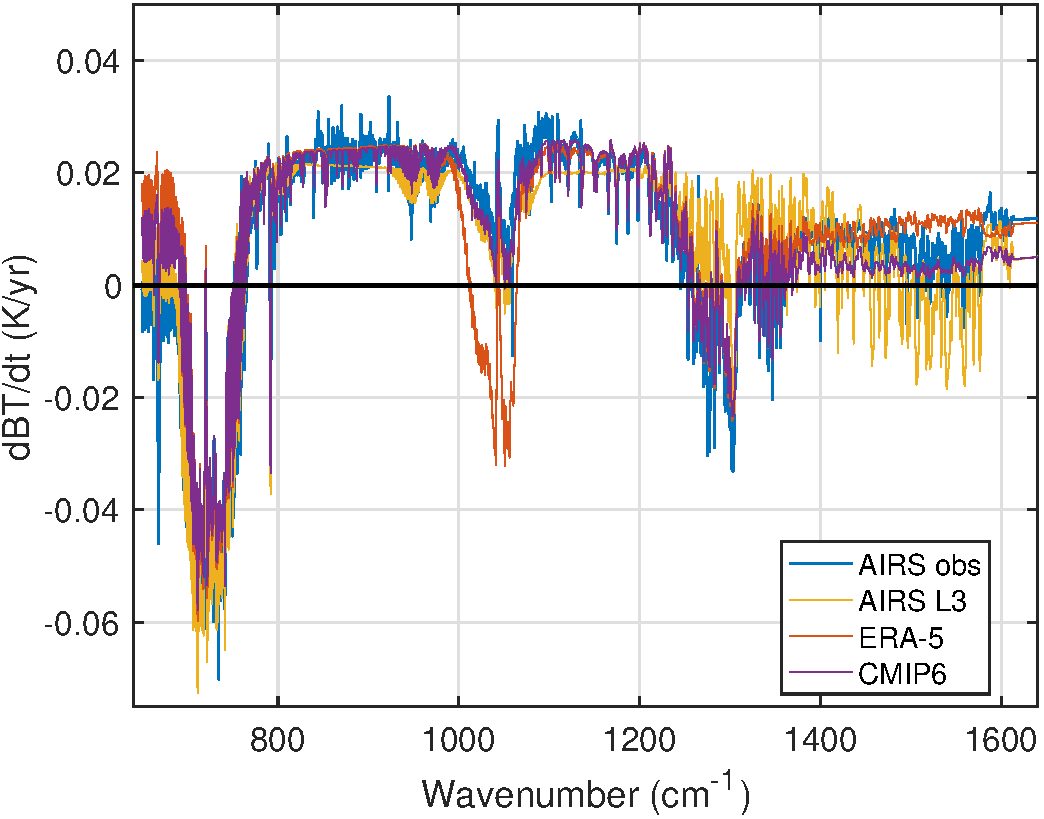
\includegraphics[width=0.75\linewidth]{Figslls/model_vs_obs_BTtrends_lls.pdf}
\end{center}
\vspace{-0.1in}
\begin{small}
\begin{itemize}
\item 19-year trends (ERA5, AIRS V7), 12-year CMIP6 trends)
\item UMBC retrieved trends (not shown) agree with AIRS observed trends
\item Trends converted to BT trends using RTA with NOAA-ESRL gas trends  
\end{itemize}
\end{small}
\end{frame}
%---------------------------------------------------------------------------------------------\
\begin{frame}
\frametitle{Surface Temperature Trend Comparisons}  
\vspace{-0.15in}
\begin{center}
%\includegraphics[width=\linewidth]{../../CONFERENCES/SunClimate2022/Strow_JPL_Apr2022/jpl_min//Figs/Png/tsurf_maps_6sources_giss.png}
\includegraphics[width=\linewidth]{SunClimate2022/tsurf_maps_6sources_giss.png}
\end{center}

\vspace{0.1in}
\footnotesize
\begin{center}
\begin{tabular}{lr}
\hline
Data Source & Spatial Correlation\\
 & (w/ UMBC)\\
\hline
CLIMCAPS AIRS & 0.82\\
GISTEMP & 0.74\\
AIRS V7 & 0.70\\
ERA-5 & 0.66\\
MERRA2 & 0.53\\
\hline
\end{tabular}
\end{center}
\end{frame}
%---------------------------------------------------------------------------------------------
\begin{frame}
\frametitle{Zonal T(z) Trends (with CMIP6 to 2014)}  
\vspace{-0.15in}
\begin{center}
%\includegraphics[width=\linewidth]{../../CONFERENCES/SunClimate2022/Strow_JPL_Apr2022/jpl_min//Figs/Pdf/zonal_trates_1to1000mbar_cmip6_newcaxis.pdf}
\includegraphics[width=\linewidth]{SunClimate2022/zonal_trates_1to1000mbar_cmip6_newcaxis.pdf}
\end{center}

\footnotesize
IR does have null space near the tropopause.  But trends change sign there as well, as they should.\\
\vspace{0.1in}
UMBC uncertainties \textasciitilde{}0.01K/year (inter-annual variability)
\end{frame}
%---------------------------------------------------------------------------------------------
\begin{frame}
\frametitle{Water Vapor Trends (with CMIP6 to 2014)}  
\vspace{-0.15in}
\begin{center}
%\includegraphics[width=\linewidth]{../../CONFERENCES/SunClimate2022/Strow_JPL_Apr2022/jpl_min//Figs/Pdf/zonal_wvrates_50to1000mbar_cmip6.pdf}
\includegraphics[width=\linewidth]{SunClimate2022/zonal_wvrates_50to1000mbar_cmip6.pdf}
\end{center}

\small
\begin{itemize}
\item UMBC a-priori of zero influencing upper-trop WV
\item Quick test using MLS trends as a-priori for UMBC upper-trop
\end{itemize}
\end{frame}

%---------------------------------------------------------------------------------------------
%\begin{frame}
%\frametitle{RH Trends (with CMIP6 to 2014)}  
%\vspace{-0.15in}
%\begin{center}
%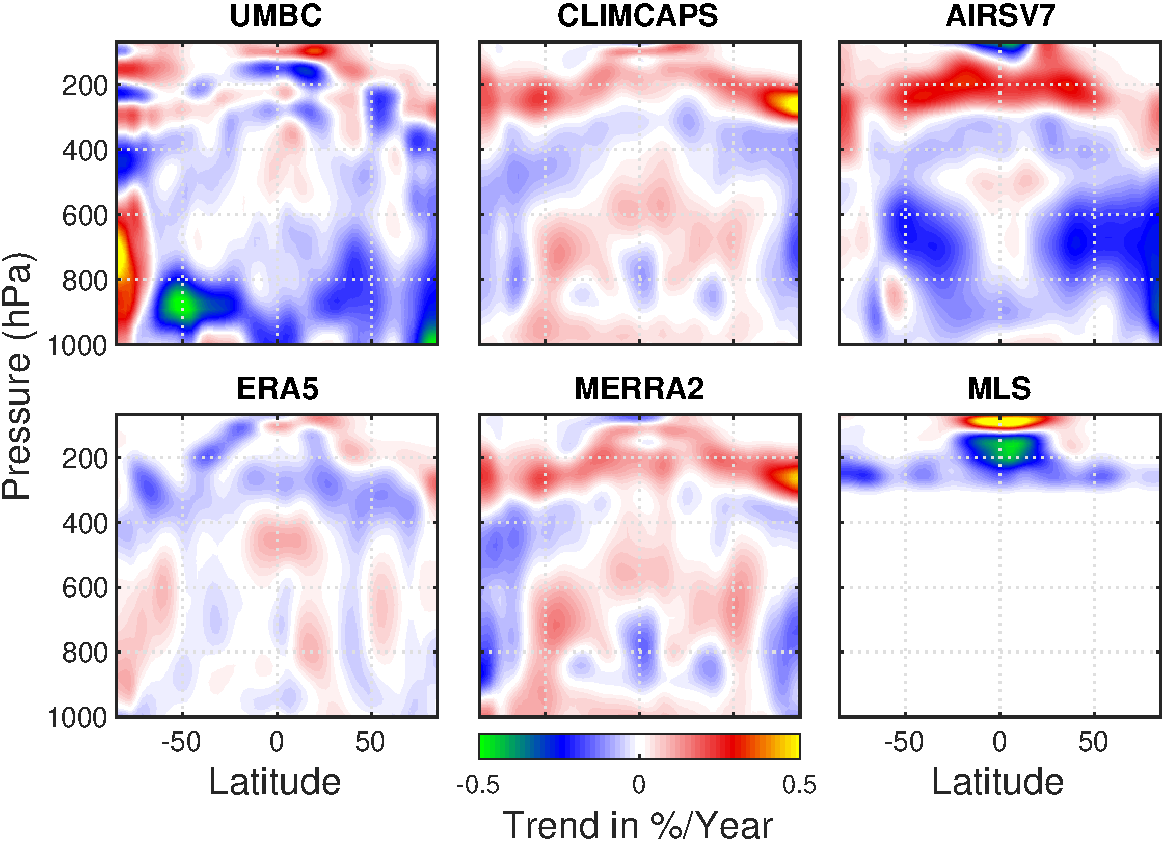
\includegraphics[width=\textwidth]{Figslls/tiled_all_N_RH_trend_withmls_start.pdf}
%\includegraphics[width=\textwidth]{test.pdf}
%\end{center}

%\small
%\begin{itemize}
%\item UMBC a-priori of zero influencing upper-trop WV
%\item Quick test using MLS trends as a-priori for UMBC upper-trop
%\end{itemize}
%\end{frame}

%\begin{frame}[label={sec:org1e985f2}]{Water Vapor Trends (with AURA-MLS: from 2004+)}
%\vspace{-0.15in}
%\begin{center}
%\includegraphics[width=\linewidth]{../../CONFERENCES/SunClimate2022/Strow_JPL_Apr2022/jpl_min//Figs/Pdf/zonal_wvrates_50to1000mbar_mls_umbc_ap_mls.pdf}
%\end{center}
%\vspace{-0.1in}
%\small
%\begin{itemize}
%\item Quick test using MLS trends as a-priori for UMBC upper-trop
%\item MLS water vapor unimportant for OLR applications
%\item Mean global \(\Delta\) RH < 0.01\%/year
%\end{itemize}
%\end{frame}
%---------------------------------------------------------------------------------------------
\begin{frame}
\frametitle{RH Vapor Trends (with CMIP6 to 2014)}  
\vspace{-0.15in}
\begin{center}
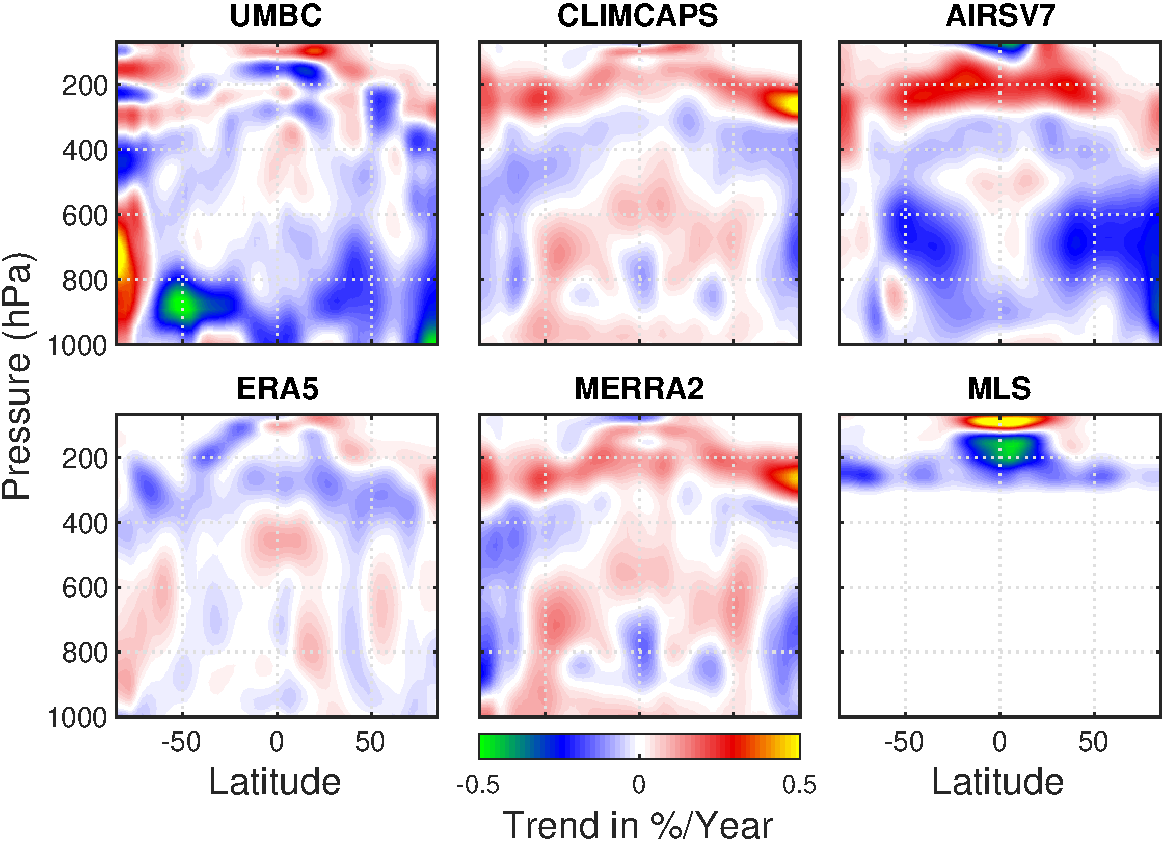
\includegraphics[width=\textwidth]{Figslls/tiled_all_N_RH_trend_withmls_start.pdf}
\end{center}

\small
\begin{itemize}
\item UMBC a-priori of zero influencing upper-trop WV
\item Quick test using MLS trends as a-priori for UMBC upper-trop
\end{itemize}
\end{frame}

%\begin{frame}[label={sec:org1e985f2}]{Water Vapor Trends (with AURA-MLS: from 2004+)}
%\vspace{-0.15in}
%\begin{center}
%\includegraphics[width=\linewidth]{../../CONFERENCES/SunClimate2022/Strow_JPL_Apr2022/jpl_min//Figs/Pdf/zonal_wvrates_50to1000mbar_mls_umbc_ap_mls.pdf}
%\end{center}
%\vspace{-0.1in}
%\small
%\begin{itemize}
%\item Quick test using MLS trends as a-priori for UMBC upper-trop
%\item MLS water vapor unimportant for OLR applications
%\item Mean global \(\Delta\) RH < 0.01\%/year
%\end{itemize}
%\end{frame}
%---------------------------------------------------------------------------------------------
\begin{frame}
\frametitle{Surface Temperature Trend Comparisons 2002/09-2014/08}  
\vspace{-0.15in}
\begin{center}
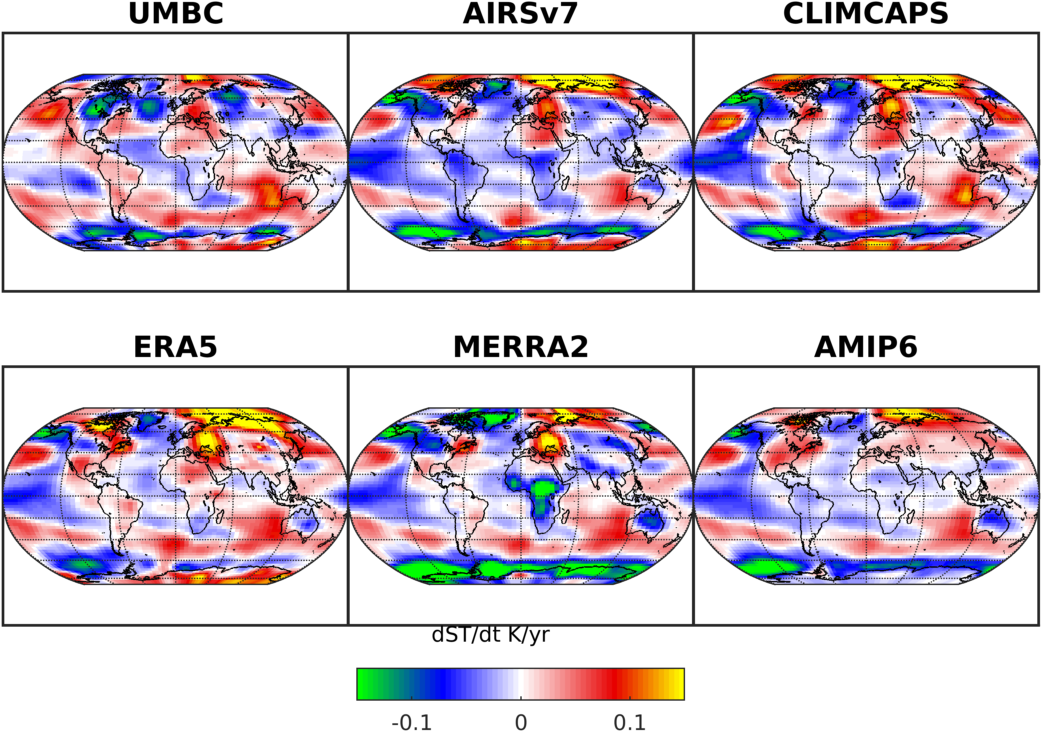
\includegraphics[width=\linewidth]{Figs2002_2014/stemp_trends_2002_2014_amip6.png}
\end{center}
\end{frame}
%---------------------------------------------------------------------------------------------
\begin{frame}
\frametitle{Zonal T(z) Trends 2002/09-2014/08}  
\vspace{-0.15in}
\begin{center}
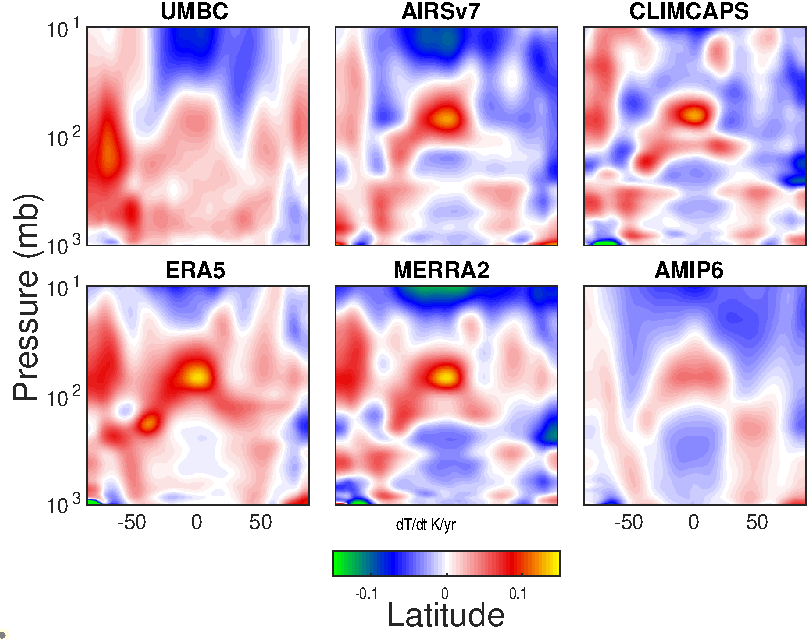
\includegraphics[width=\linewidth]{Figs2002_2014/tz_trends_2002_2014.pdf}
\end{center}
\end{frame}
%---------------------------------------------------------------------------------------------
\begin{frame}
\frametitle{WV(z) Fractional Trends 2002/09-2014/08}  
\vspace{-0.15in}
\begin{center}
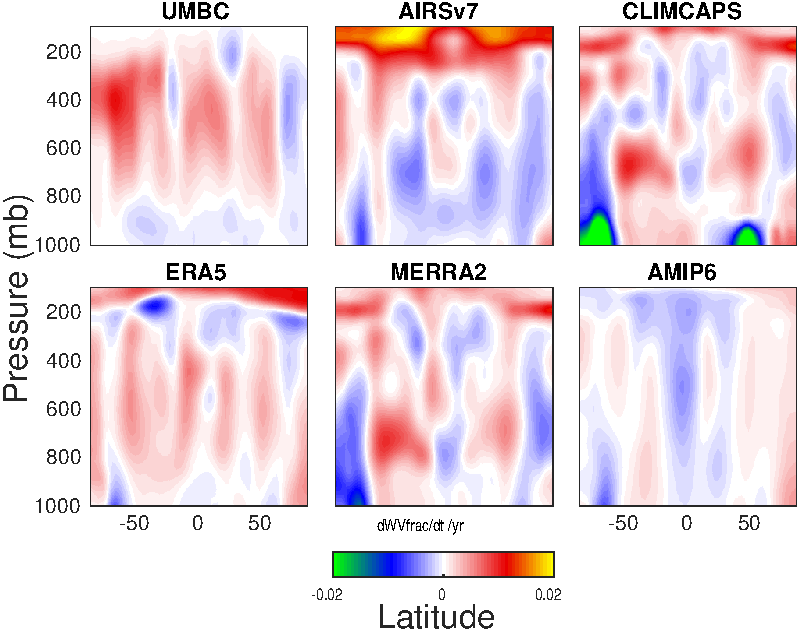
\includegraphics[width=\linewidth]{Figs2002_2014/wvfrac_trends_2002_2014.pdf}
\end{center}
\end{frame}

%---------------------------------------------------------------------------------------------
\begin{frame}
\frametitle{RH(z) Trends 2002/09-2014/08}  
\vspace{-0.15in}
\begin{center}
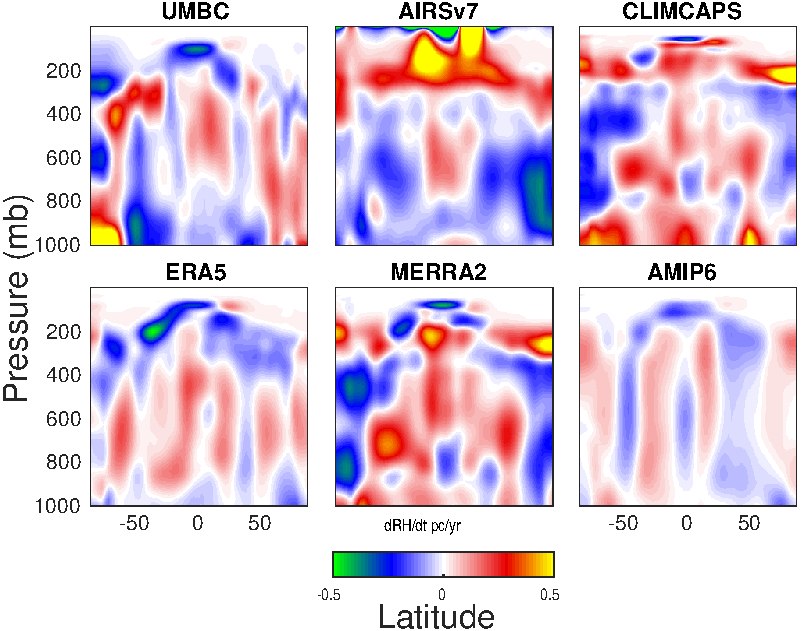
\includegraphics[width=\textwidth]{Figs2002_2014/RHz_trends_2002_2014.pdf}
\end{center}
\end{frame}
%---------------------------------------------------------------------------------------------
\begin{frame}
\frametitle{Climate Feedback Estimation from Trend Retrievals}  
  \vspace{-0.2in}
  \begin{columns}[T]
    \begin{column}{0.5\columnwidth}
      \begin{block}{\footnotesize \(\lambda\) WV}
        \vspace{-0.15in}
        \begin{center}
          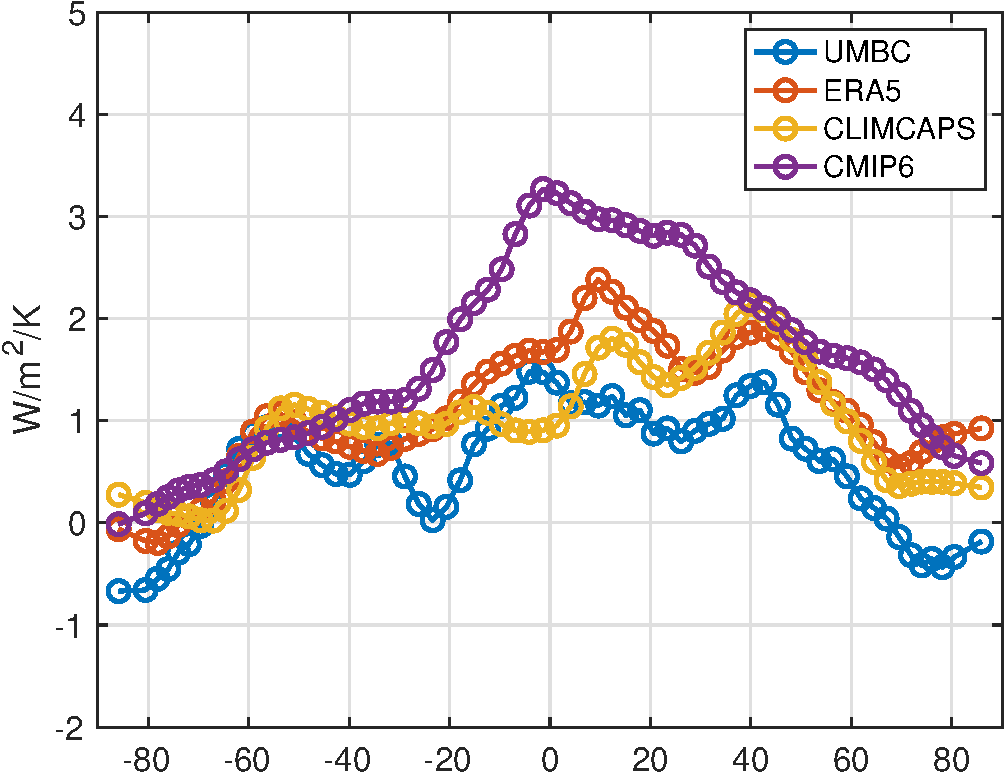
\includegraphics[width=0.85\linewidth]{Figslls/wv_lambda.pdf}
        \end{center}
      \end{block}
    \end{column}


    \begin{column}{0.5\columnwidth}
      \begin{block}{\footnotesize \(\lambda\) Lapse Rate}
        \vspace{-0.15in}
        \begin{center}
          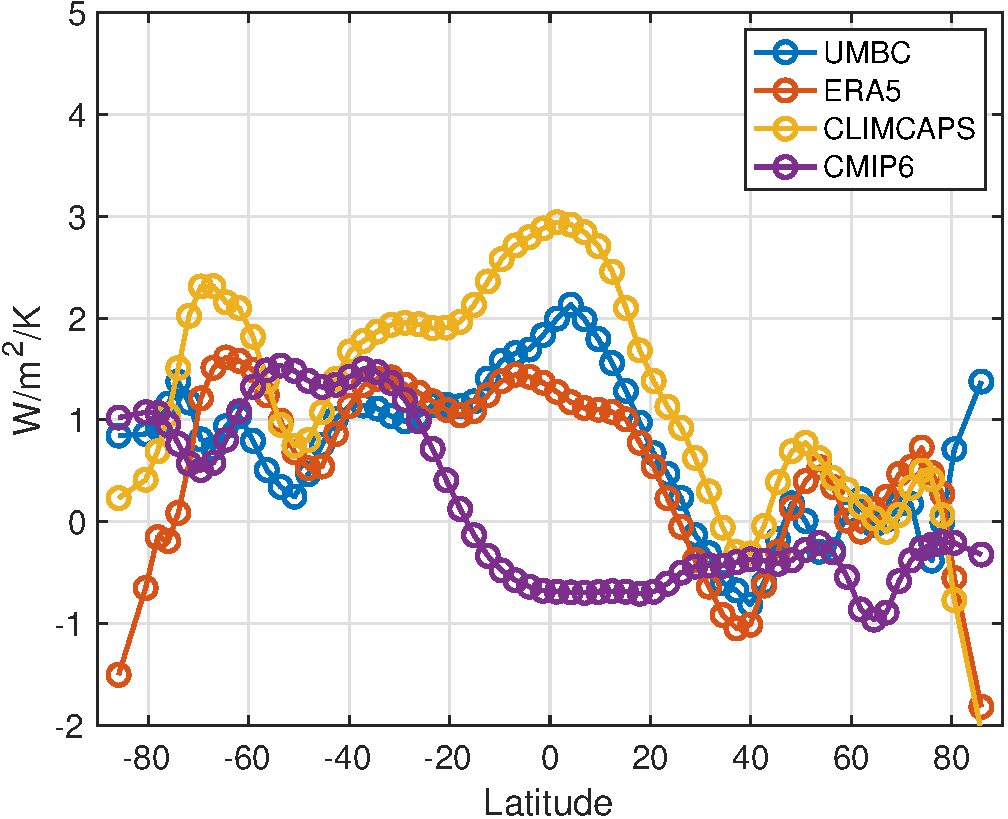
\includegraphics[width=0.85\linewidth]{Figslls/lapse_lambda.pdf}
        \end{center}
      \end{block}
    \end{column}
  \end{columns}

  \begin{columns}[T]
    \begin{column}{0.5\columnwidth}
      \vspace{-0.2in}
      \begin{block}{\footnotesize $\lambda$ WV + Lapse Rate}
        \vspace{-0.15in}
        \begin{center}
          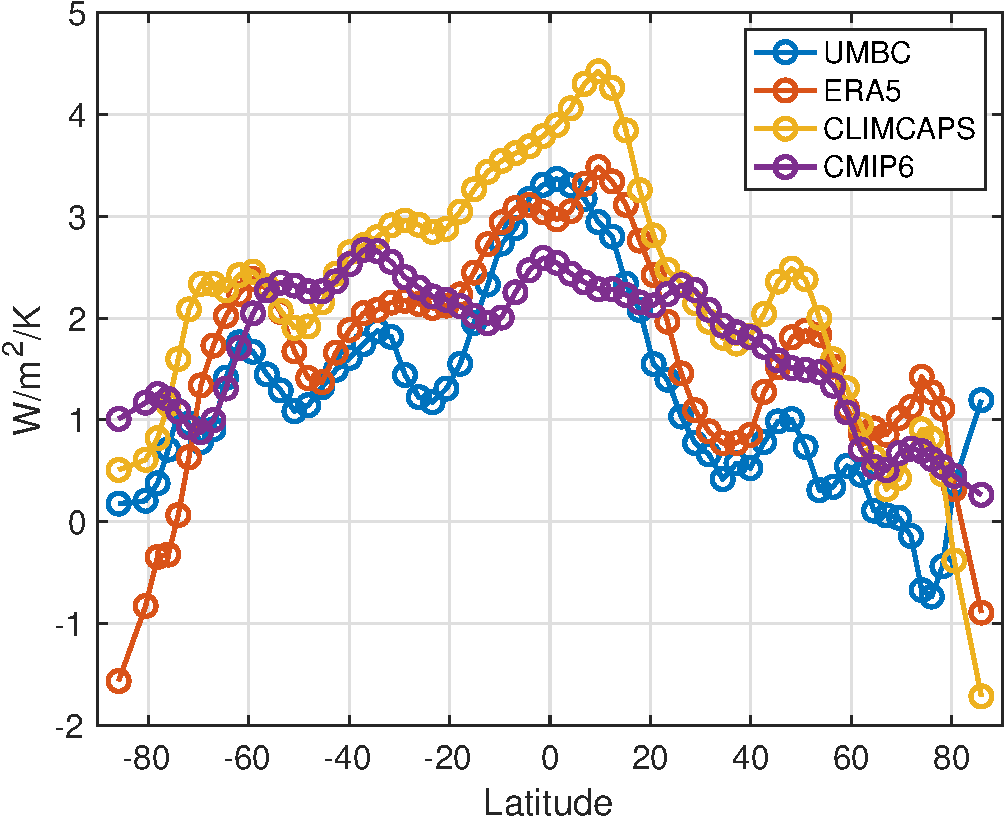
\includegraphics[width=0.85\linewidth]{Figslls/wv_plus_lapse_lambda.pdf}
        \end{center}
      \end{block}
    \end{column}

    \begin{column}{0.5\columnwidth}
      \begin{footnotesize}
        \begin{itemize}
        \item CMIP period ends 2014, others end in 2021
        \item OLR differences computed from obs trends
        \item Cannot use MERRA2 due to poor surface T trends
        \item Hard to separate feedbacks, does it matter?
        \end{itemize}
      \end{footnotesize}
    \end{column}
  \end{columns}
\end{frame}
%---------------------------------------------------------------------------------------------
\begin{frame}
\frametitle{OLR Clear Sky Trends from AIRS (UMBC version)}  
\vspace{-0.1in}

\begin{columns}
\begin{column}{0.5\columnwidth}
\begin{block}{\small Total \(\Delta\) OLR (clear) over 19 Years}
\vspace{-0.1in}
\begin{center}
%\includegraphics[width=\linewidth]{../../CONFERENCES/SunClimate2022/Strow_JPL_Apr2022/jpl_min//Figs/Png/ceres_clear_and_cld_19yrold_vs_umbc.png}
\includegraphics[width=\linewidth]{SunClimate2022/ceres_clear_and_cld_19yrold_vs_umbc.png}
\end{center}
\end{block}
\end{column}

\begin{column}{0.5\columnwidth}
\begin{block}{\small Components from AIRS Trends}
\vspace{-0.1in}
\begin{center}
%\includegraphics[width=\linewidth]{../../CONFERENCES/SunClimate2022/Strow_JPL_Apr2022/jpl_min//Figs/Pdf/umbc_olr_components.pdf}
\includegraphics[width=\linewidth]{SunClimate2022/umbc_olr_components.pdf}
\end{center}
\end{block}
\end{column}
\end{columns}

\vspace{-0.05in}

\begin{itemize}
\item UMBC clear closest to CERES All-Sky (but not perfect)
\item Hints for these differences seen in cloud forcing PDFs (in two slides)
\end{itemize}
\end{frame}
%---------------------------------------------------------------------------------------------
\begin{frame}
\frametitle{Summary and Future}  
\begin{itemize}

\item Hyperspectral IR observations are a unique dataset to monitor
  and understand climate change, for weather prediction and
  reanalysis, and to evaluate climate models

\item Hyperspectral IR radiances provide insights into the physics of
  the climate system that are not possible using broadband
  observations

\item We are starting to successfully merge hyperspectral IR radiances
  from different instruments which is critical for climate monitoring
  (GPSRO, MLS, MODIS/VIIRS)

\item We will continue to improve these merged products using more
  sophisticated approaches and including additional observations

\item But we need to keep these hyperspectral IR instruments alive and
  stable for as long as technically possible and continue to produce
  climate-level calibrated radiances

\end{itemize}
\end{frame}
%---------------------------------------------------------------------------------------------
\begin{frame}
\frametitle{L1b radiance Stability}  
\vspace{-0.35in}
\begin{center}
\includegraphics[width=1.01\linewidth,page={14}]{Slides_to_Sergio.pdf}
\end{center}
\end{frame}

\begin{frame}
\frametitle{Summary}  
\vspace{-0.35in}
\begin{center}
\includegraphics[width=1.01\linewidth,page={17}]{Slides_to_Sergio.pdf}
\end{center}
\end{frame}

\begin{frame}
\frametitle{Future}  
\vspace{-0.35in}
\begin{center}
\includegraphics[width=1.01\linewidth,page={18}]{Slides_to_Sergio.pdf}
\end{center}
\end{frame}

\end{document}


%------------------ Commented Out Slides
%---------------------------------------------------------------------------------------------
%\begin{frame}
%   \frametitle{Hyperspectral Infrared Satellite Sounders}

% \begin{columns}
% \begin{column}{0.55\columnwidth}
% \begin{block}{}
%   \begin{itemize}
%   \item 
%   \item 
%   \end{itemize}
% \end{block}
% \end{column}

% \begin{column}{0.55\columnwidth}
% \begin{block}{}
%   \begin{itemize}
%   \item 
%   \item 
%   \end{itemize}
% \end{block}
% \end{column}
% \end{columns}
  
% \end{frame}


%---------------------------------------------------------------------------------------------
% \begin{frame}
% \frametitle{OLR in the IR $\rightarrow$ Far-IR}  
% \begin{block}{}

% \vspace{-0.1in}
% \begin{columns}

% \begin{column}{0.55\columnwidth}
% \begin{block}{}
% \vspace{-0.1in}
% \begin{center}
% \includegraphics[width=\linewidth]{NEWFIGS/image_spectralOLR.png}
% \end{center}
% \end{block}
% \end{column}

% \begin{column}{0.55\columnwidth}
% \begin{block}{}
% \begin{itemize}
% \item Far-IR WV emission dominates atmospheric cooling, esp. in descending tropical regions
% \item AIRS observed mid-IR WV has sensitivity where (WV) OLR is large in far-IR
% \item Allows computation of feedbacks from AIRS retrievals using computed OLR driven by mid-IR WV retrievals
% \end{itemize}
% \end{block}
% \end{column}

% \end{columns}

% \end{block}
% \end{frame}
% ---------------------------------------------------------------------------------------------

%---------------------------------------------------------------------------------------------
% \begin{frame}
% \frametitle{Changes to Severe Weather Storms}  
% \vspace{-0.35in}
% \begin{center}
% \includegraphics[width=1.01\linewidth,page={6}]{Slides_to_Sergio.pdf}
% \end{center}
% \end{frame}


% %---------------------------------------------------------------------------------------------
% \begin{frame}[shrink=2]
% \frametitle{Radiative Transfer codes : Accuracy vs Speed}
% \vspace{-0.1in}
% \begin{columns}

% \begin{column}{0.55\columnwidth}
% \begin{block}{Line by line codes : accuracy}
%   \begin{itemize}
%   \item Use latest HITRAN/GEISA databases; accurate; too slow for operational use
%   \item GENLN2 (Dave Edwards) - 15 um \cd line mixing from L.Strow
%   \item LBLRTM (AER) WV,N2/O2/other gases continuum, \cd/\methane line mixing, spans MW to UV
%   \item \textcolor{red}{kCARTA (UMBC)} \emph{HITRAN (2020), MT-CKD 3.2,\cd/\methane linemixing from LBLRTM, 
%         605-2830 \wn at 0.0025 \wn resolution (25 sec), 15-44000 \wn (5 min), jacobians, 
%         fluxes, scattering}
%   \end{itemize}
% \end{block}
% \end{column}

% \begin{column}{0.55\columnwidth}
% \begin{block}{Fast Models : speed}
%   \begin{itemize}
%   \item Parametrized fast codes for clear sky cloud clearing retrievals
%   \item We use 49 regression profiles to span a variety of Earth climates; ECMWF has eg 25000
%   \item \textcolor{red}{SARTA (UMBC)} \emph{used by NASA and NOAA for operational L2 retrievals of AIRS/CrIS, IASI}
%   \item PCRTM (NASA Langley)
%   \item RTTOVS (ECMWF) Data Assimilation
%   \item Sigma IASI (U. of Basilicata, Italy) 
%   \end{itemize}
% \end{block}
% \end{column}
% \end{columns}
% \end{frame}
% %---------------------------------------------------------------------------------------------
% \begin{frame}[shrink=2]
% \frametitle{Radiative Transfer Models (con'd)}
% \vspace{-0.1in}
% \begin{columns}

% \begin{column}{0.55\columnwidth}
% \begin{block}{Spectroscopy}
%   \begin{itemize}
%   \item HITRAN released every 4 years
%   \item H2020 : self consistent changes to O3 line intensities (MW to UV) $\Delta BT(K) \sim 0.5K$ at 10 um
%   \item Uncertainty estimates : $\delta(BT) \sim$ 0.2 K at TOA  
%   \item Line mixing models; speed dependent Voigt line shapes used in other spectral regions
%   \item AER : new WV continuum in Fall 2022 (TIR region); H2020 \cd/\methane linemixing
%   \item GEISA database (France) is very similar to HITRAN

%   \end{itemize}
% \end{block}
% \end{column}

% \begin{column}{0.55\columnwidth}
% \begin{block}{Non local thermodynamic equilibrium}
%   \begin{itemize}
%   \item NLTE mostly affects the 4.3 um \cd band (nadir sounding)
%   \item Manuel Lopez Puertas (Granada, Spain) has developed models upper atmosphere NLTE vibrational temperatures
%   \item UMBC developed a fast model using this database
%   \item We don't worry too much about strat/meso temperatures and atmospheric concentrations (cannot see with nadir sounders)
%   \end{itemize}
% \end{block}
% \end{column}
% \end{columns}
% \end{frame}


% %---------------------------------------------------------------------------------------------
% \begin{frame}[shrink=2]{Radiative Transfer Models (con'd)}
% \vspace{-0.1in}
% \begin{columns}

% \begin{column}{0.55\columnwidth}
% \begin{block}{Surface properties}
%   \begin{itemize}
%   \item Ocean emissivity : Masuda model (1988,2006) $\epsilon(\nu,wspeed)$
%   \item Land Emissivity : Dan Zhou (NASA Langley) and CAMEL (U. Wisc) $\epsilon(\nu,YY/MM)$
%   \end{itemize}
% \end{block}

% \begin{block}{Scattering}
%   \begin{itemize}
%   \item DISORT (Stamnes et. al. 1988) : Very accurate, but slow
%   \item Parameterization for LongWave Scattering (Chou et. al 1999) : Very fast, about 2 K errors
%   %\item Successive Orders of Scattering : mostly used for NIR/Vis (to my knowledge)
%   \item PCLSAM fix (Tang. et. al 2018) : Needs more work
%   \end{itemize}
% \end{block}
% \end{column}

% \begin{column}{0.55\columnwidth}
% \begin{block}{Clouds and Aerosols (dme $\ge$ 3 um)}
%   \begin{itemize}
%   \item Complex cloud models (Maximum Random Overlap) give smooth heating profiles, multiple sub pixels are computationally costly
%   \item Simple cloud models (TwoSlab) are fast and quite accurate, spikes at cloud slab boundaries
%   \item RRTM (AER) has in-built fast RTA for flux calculations, handles scattering, 3-4 gaussian angles
%   \item ecRad (Robin Hogan, ECMWF) developed flux model for ECWMF
%   \end{itemize}
% \end{block}
% \end{column}
% \end{columns}
% \end{frame}
% %---------------------------------------------------------------------------------------------
% \begin{frame}[shrink=2]
% \frametitle{Operational Retrievals}
% \vspace{-0.11in}
% \begin{columns}

% \begin{column}{0.55\columnwidth}
% \begin{block}{Typical Hyperspectral Sounder}
%   \begin{itemize}
%   \item Atmospheric Infrared Sounder, operational since 2002/09
%   \item Diffraction grating instrument, 2378 channels, 500 pristine channels 
%         (Strow/Machado AMT 2018) of resolution about 0.5-2 cm-1, 15 km diameter footprint
%   \item 1.30 am/pm equator crossing time, twice daily views of Earth, 16 day repeat cycle
%   \item 90 xtrack x 135 atrack spectra every 6 minutes
%   \item Roughly \textcolor{red}{2.92 million  allsky spectra daily x 20 years!}
%   \end{itemize}
% \end{block}
% \end{column}

% \begin{column}{0.55\columnwidth}
% \begin{block}{Typical Operational Retrieval}
%   \begin{itemize}
%     \item Cloud clearing process 
%        \begin{itemize}
%           \item reduces spatial resolution from 15 km to 3x3 or 45 km
%           \item ``increases'' spectral noise, and hence retrieval uncertainty
%           \item fails when scenes are uniform eg MBL, dust, clear
%        \end{itemize}
%     \item \textcolor{red}{T(z), WV(z), surface temp, trace gases, clouds, emissivity}
%     \item AIRS v7 : neural network first guess, 2 sec/FOR, Lots of QA, 
%     \item NOAA CLIMCAPS MERRA2 first guess, simpler QA, 0.7 sec/FOR
%     \item Single Footprint? Artificial Intelligence?
% %    \begin{itemize}
% %      \item EUMETSAT does hole hunting to look for clear scenes
% %      \item Regression based allsky retrievals (Bill Smith UWisc/Hampton U)
% %      \item Single footprint allsky retrievals (JPL Irion, Langley Liu, UMBC)
% %      \item Artificial Intelligence allsky retrievals (NOAA Maddy/Boukabara)
% %    \end{itemize}
%   \end{itemize}
% \end{block}
% \end{column}
% \end{columns}
% \end{frame}

% %---------------------------------------------------------------------------------------------
% \begin{frame}
% \frametitle{Impact of Spectral Uncertainties ($\Delta$ (BT) at TOA)}  

% \begin{block}{Perturbations to}
% GEISA vs HITRAN, wavenumber unc, pressure line shift unc \newline $\rightarrow$ $\le$ 0.1 K RMS differences
% \end{block}

% \vspace{-0.1in}
% \begin{columns}

% \begin{column}{0.55\columnwidth}
% \begin{block}{Spectroscopic Database}
% LBLTMv12.8 15 \um \cd line mixing versus \newline
% LBLRTM 12.4 (red) UMBCLBL (blue) \newline
% \textcolor{red}{But integral over wavenumber should give similar fluxes}
% \end{block}
% \end{column}

% \begin{column}{0.55\columnwidth}
% \begin{figure}
% \begin{center}
% %\includegraphics[width=0.45\textwidth]{../../SUBMITPAPERS/PAPER1_KCARTA/GEISA_HTRAN/hitran_geisaV2.pdf}
% %\includegraphics[width=1.005\textwidth]{../../SUBMITPAPERS/PAPER1_KCARTA/GEISA_HTRAN/co2_linemix_flavorsV2.pdf}
% \includegraphics[width=1.005\textwidth]{NEWFIGS/co2_linemix_flavorsV2.pdf}
% \end{center}
% \end{figure}
% \end{column}
% \end{columns}
% \end{frame}
%---------------------------------------------------------------------------------------------
%---------------------------------------------------------------------------------------------
% \begin{frame}
% \frametitle{Follow-On Sensor: SNPP CrIS 8-Year Trends}  
% \begin{center}
% %\includegraphics[width=0.8\linewidth]{../../CONFERENCES/SunClimate2022/Strow_JPL_Apr2022/jpl_min//Figs/Pdf/cris_dbt_clear_all_lats_lwmw_annotated.pdf}
% \includegraphics[width=0.8\linewidth]{SunClimate2022/cris_dbt_clear_all_lats_lwmw_annotated.pdf}
% \end{center}
% \vspace{-0.1in}
% \footnotesize Clear ocean scenes \\
% \footnotesize Less "hash" due to nature of FTS instrumentation
% \end{frame}

%%% Local Variables:
%%% mode: latex
%%% TeX-master: t
%%% End:
